\documentclass{beamer}
%\usetheme{Darmstadt}
\usetheme{progressbar}
%\usecolortheme{default}
%\usecolortheme{crane}
\usepackage[utf8]{inputenc}
\usepackage[czech]{babel}
\usepackage{graphicx}
\usepackage{multicol}
\usepackage{xcolor}
\title[Skoleni Gitu]{Skoleni Gitu}
\subtitle[E-solutions s.r.o.]{E-solutions s.r.o.}
\author[Ondrej Sika]{Ondrej Sika \texttt{<ondrej@ondrejsika.com>}}
\date[12. 9. 2016]{12. 9. 2016}

\begin{document}

% titulní stránka
% (název prezentace, autor, datum...)

%background
%\usebackgroundtemplate{\includegraphics[width=\paperwidth]{background.png}}

\begin{frame}
  \titlepage
\end{frame}

% osnova prezentace
% (většinou se pro délku vypouští)

%\begin{frame}
%  \tableofcontents
%\end{frame}

% obsah prezentace
% (používají se klasické sekce)

\section{Jízdenky Českých drah}

\begin{frame}
	\frametitle{Současná podoba jízdenek}
	\begin{center}
		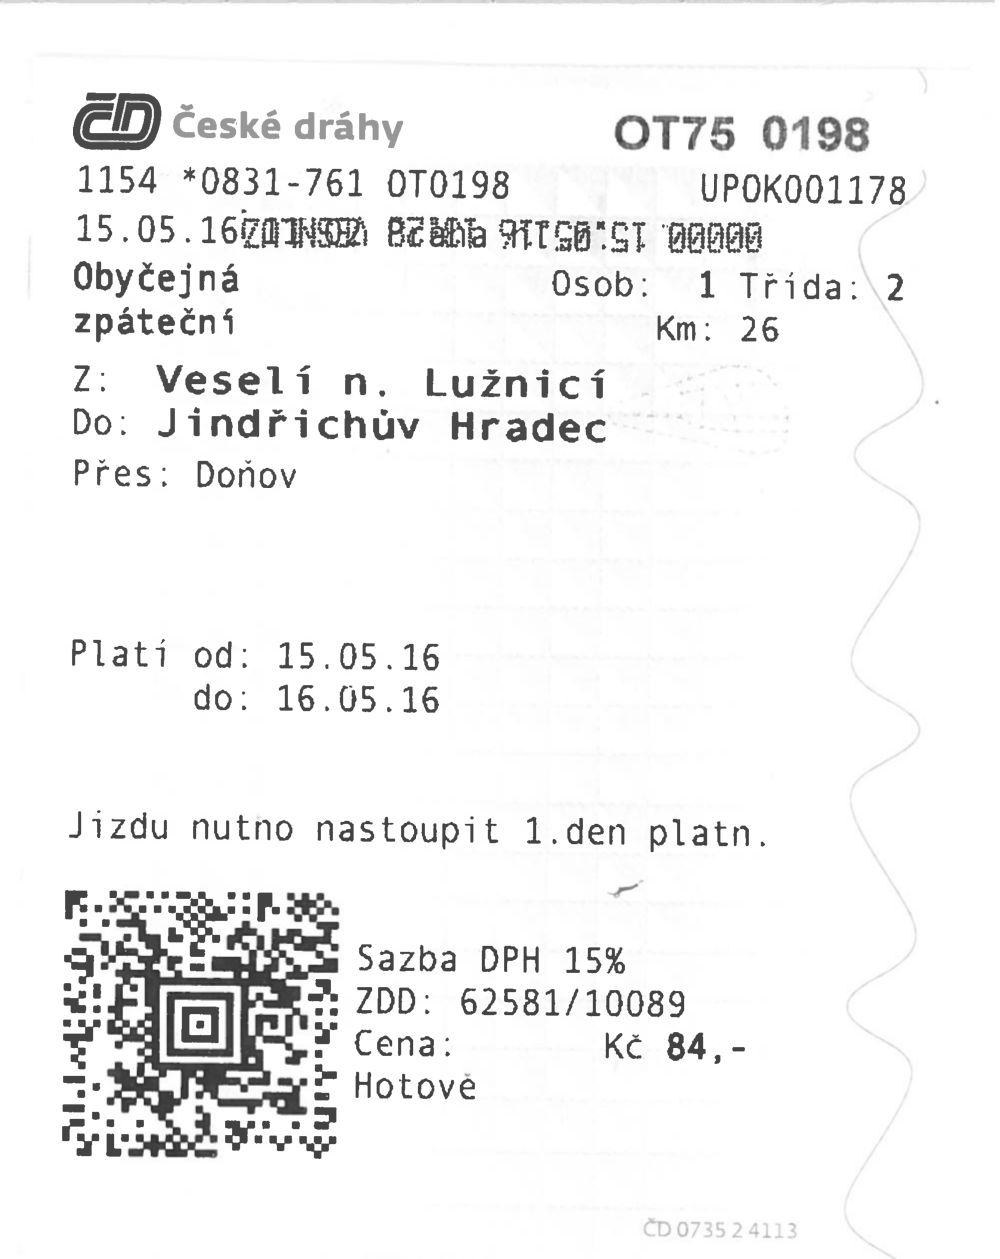
\includegraphics[scale=0.16]{./images/0033_0010.png}
	\end{center}
\end{frame}

\begin{frame}
	\frametitle{ISO/IEC 24778:2008 (Aztécký kód)${ }^{[1]}$}
	%\begin{center}
		\begin{multicols}{2}
			
\includegraphics[scale=0.25]{./images/Aztec_Code_Scheme.png}
			\newpage
			\texttt{\ }\texttt{\ }\texttt{\ }\texttt{\ }\color{black}{Pevně definované bity}\\
			\texttt{\ }\texttt{\ }\texttt{\ }\texttt{\ }\color{red}{Struktury}\\
			\texttt{\ }\texttt{\ }\texttt{\ }\texttt{\ }\color{green}{Nastavení (velikost, mod)}\\
			\texttt{\ }\texttt{\ }\texttt{\ }\texttt{\ }\color{blue}{Data + Reed-Solomon}\\
			\texttt{\ }\texttt{\ }\texttt{\ }\texttt{\ }\color{gray}{Začátek dvojřádku}
		\end{multicols}
	%\end{center}
\end{frame}

\begin{frame}
	\frametitle{Jízdenka 0033\_0010}
	\color{black}
	České dráhy používají od roku 2012\\
	\begin{center}
		
\includegraphics[scale=2]{./images/aztec/0033_0010.png}
	\end{center}
\end{frame}

\begin{frame}
	\frametitle{Data na jízdence}
	\color{black}
	Binární blob proměnlivé délky (okolo 96B)\\
	Nešifrované údaje\\
	\texttt{\ }\\
	\texttt{23434430 31C2830E 29C39BC2 9A040000\\
	        11C2B10C 00C29129 C3A4C2B8 2EC381C3\\
	        A440C2B4 44530006 150A2500 00000000\\
	        20C381C3 A4400000 000040C3 81C3A440\\
	        10C28553 003AC288 53000100 000000C3\\
	        90200000 0A}
\end{frame}

\begin{frame}
	\frametitle{Data na jízdence}
	\color{black}
	Zvýrazněné prvky (viz další slajd)\\
	Fixní pořadí, proměnlivé offsety\\
	\texttt{\ }\\
	\texttt{\color{red}{23434430 31}\color{black}{C2830E 29C39BC2} \color{cyan}{9A040000}\\
	        \color{black}{11C2B10C 00C29129 C3A4C2B8 2E}\color{orange}{C381}\color{blue}{C3\\
	        A440}\color{green}{C2B4 4453}\color{black}{0006 150A2500 00000000\\
	        20}\color{orange}{C381}\color{blue}{C3 A440}\color{black}{0000 000040}\color{orange}{C3 81}\color{blue}{C3A440}\\
	        \color{magenta}{10C28553}	\color{black} 00\color{olive}{3AC288 53}\color{black}{000100 000000C3\\
	        90200000 0A}}
\end{frame}

\begin{frame}
	\frametitle{Význam některých struktur}
	\texttt{\color{red}{2343443031}} \color{black} - "\#CD01" - identifikátor dopravce\\
	\texttt{\color{cyan}{9A040000}} \color{black} - datum + 2B 0x00\\
	\texttt{\color{orange}{C381}} \color{black} - kontrolní součet, vždy před oddělovačem\\
	\texttt{\color{blue}{C3A440}} \color{black} - globálně konstantní oddělovač (3x)\\
	\texttt{\color{green}{C2B44453}} \color{black} - ID Prodejní stanice (=Praha hl.n.)\\
	\texttt{\color{magenta}{10C28553}} \color{black} - ID Odkud (=Veselí nad Lužnicí)\\
	\texttt{\color{olive}{3AC28853}} \color{black} - ID Kam (=Jindřichův Hradec)\\
	\texttt{\color{black}{XXXXXXXX}} - neznámý význam a padding
\end{frame}

\begin{frame}
	\frametitle{Nedekódované údaje}
	\begin{itemize}
		\item Datum a čas (částečně)
		\item ID jízdenky, pokladny/pokladní, jízdenkové řady
		\item Počet osob
		\item Slevy (IN25/50/100, studentská, zpáteční,...)
		\item Extra (kolo, pes, místenka,...)
	\end{itemize}
\end{frame}

\begin{frame}
	\frametitle{Nejisté údaje}
	\color{black}
	Možná to v kódu uložené je, možná ne
	\begin{itemize}
		\item Kilometráž
		\item Cena
		\item Trať (Praha -- Č. Budějovice přes Tábor/Písek)
	\end{itemize}
\end{frame}

\begin{frame}
	\frametitle{Jízdenka z webu ČD}
	\color{black}
	Při online nákupu si lze vytisknout jízdenku doma\\
	Kod je mnohem obsáhlejší a NEdodržuje výše popsanou strukturu\\
	Obsahuje navíc údaje o přepravovaném:
	\begin{itemize}
		\item Jméno Příjmení
		\item ID dokladu (OP, pas, řidičák, zbroják)
		\item Číslo vlaku, trať
		\item Kontroluje se online (sync DB každých pár minut)
	\end{itemize}
	Pravděpodobně šifrováno (ÚOOÚ)?
\end{frame}

\begin{frame}
	\frametitle{Zdroje}
	\color{black}
	Databáze (SQLite) jízdenek a scripty okolo: \url{http://brmcd.s0c4.net/}\\
	\texttt{\ }\\
	\tiny{[1] \url{https://upload.wikimedia.org/wikipedia/commons/1/1a/Aztec_Code_Scheme.png}}
\end{frame}

\end{document}
